\documentclass{anstrans}

%how do i cite wikipedia? line11 body.tex
%bibliography issues
%get rid of 'no need for land purchase'





% things to consider
% maybe get rid of the environmentalists? and melt them into 'local' or 'public'
%clinton has an aquifer underneath..
% state that repository is done by DOE or exelon?
%specify who is in charge
%  ---- generally more precisely describe the proposed case 
% who what when where why
% wouldn't 'net cost' include everything from new above-ground facility and 
% no need for additional land purchase?
%       what about assessing those criterias only in a social / polical way
%          and the economic aspects of those are considered in the net cost section?
% what to write about the base case ( compare it to Yucca Mountain procedure or what?)
% datadtatdatdadatadta



%meeting Oct. 11/2016

% be explicit about the metric 
% have a statement saying and we developed metrics for this
% combine abstract and body to paper.tex
% have a main tex that contains all structures.
% \input{nameoffile}
% paper about wrting a paper
% abstract: motivation and results and talk about my contributions
% introduction: rest to understand the paper (background etc) 
% ans transactions guidelines
% methodology : how to reproduce my results
       %exactly everything to replicate result
       %to do the distance analysis, I used this equation and this code:
       

% results and discussion : everything learned
% cite things!!!! - wikipedia, this data was scraped from public information
% mention why the weights of staekholders is the way they are.
% utilities do not have much incentive to do so.
% cost of treatment licenses
% 'skilled worker', existence.

%consider Dr.Singers:
	% Don't assume money is all there
	%reduce amount of money so they can be offered to the stakeholder
	



%%%% packages and definitions (optional)
\usepackage{graphicx} % allows inclusion of graphics
\usepackage{graphics}
\usepackage{booktabs} % nice rules (thick lines) for tables
\usepackage{microtype} % improves typography for PDF



\newcommand{\SN}{S$_N$}
\renewcommand{\vec}[1]{\bm{#1}} %vector is bold italic
\newcommand{\vd}{\bm{\cdot}} % slightly bold vector dot
\newcommand{\grad}{\vec{\nabla}} % gradient
\newcommand{\ud}{\mathop{}\!\mathrm{d}} % upright derivative symbol
\graphicspath{ {images/} }

\title{Benefits of Siting a Borehole Repository on Non-Operating Nuclear 
Facility}
\author{Jin Whan Bae, William Roy, Kathryn Huff}

\institute{
Dept. of Nuclear, Plasma, and Radiological Engineering, University of Illinois at Urbana-Champaign
\and
Urbana, IL
}
\email{jbae11@illinois.edu}


%%%% Acronym support

\usepackage[acronym,toc]{glossaries}
%\newacronym{<++>}{<++>}{<++>}
\newacronym[longplural={metric tons of heavy metal}]{MTHM}{MTHM}{metric ton of heavy metal}
\newacronym{ABM}{ABM}{agent-based modeling}
\newacronym{ACDIS}{ACDIS}{Program in Arms Control \& Domestic and International Security}
\newacronym{AHTR}{AHTR}{Advanced High Temperature Reactor}
\newacronym{ANDRA}{ANDRA}{Agence Nationale pour la gestion des D\'echets RAdioactifs, the French National Agency for Radioactive Waste Management}
\newacronym{ANL}{ANL}{Argonne National Laboratory}
\newacronym{API}{API}{application programming interface}
\newacronym{ASME}{ASME}{American Society of Mechanical Engineers}
\newacronym{ATWS}{ATWS}{Anticipated Transient Without Scram}
\newacronym{BDBE}{BDBE}{Beyond Design Basis Event}
\newacronym{BIDS}{BIDS}{Berkeley Institute for Data Science}
\newacronym{CAFCA}{CAFCA}{ Code for Advanced Fuel Cycles Assessment }
\newacronym{CDTN}{CDTN}{Centro de Desenvolvimento da Tecnologia Nuclear}
\newacronym{CEA}{CEA}{Commissariat \`a l'\'Energie Atomique et aux \'Energies Alternatives}
\newacronym{CI}{CI}{continuous integration}
\newacronym{CNEN}{CNEN}{Comiss\~{a}o Nacional de Energia Nuclear}
\newacronym{CNERG}{CNERG}{Computational Nuclear Engineering Research Group}
\newacronym{COSI}{COSI}{Commelini-Sicard}
\newacronym{COTS}{COTS}{commercial, off-the-shelf}
\newacronym{CSNF}{CSNF}{commercial spent nuclear fuel}
\newacronym{CTAH}{CTAHs}{Coiled Tube Air Heaters}
\newacronym{CUBIT}{CUBIT}{CUBIT Geometry and Mesh Generation Toolkit}
\newacronym{CURIE}{CURIE}{Centralized Used Fuel Resource for Information Exchange}
\newacronym{DAG}{DAG}{directed acyclic graph}
\newacronym{DANESS}{DANESS}{Dynamic Analysis of Nuclear Energy System Strategies}
\newacronym{DBE}{DBE}{Design Basis Event}
\newacronym{DESAE}{DESAE}{Dynamic Analysis of Nuclear Energy Systems Strategies}
\newacronym{DHS}{DHS}{Department of Homeland Security}
\newacronym{DOE}{DOE}{Department of Energy}
\newacronym{DRACS}{DRACS}{Direct Reactor Auxiliary Cooling System}
\newacronym{DRE}{DRE}{dynamic resource exchange}
\newacronym{DSNF}{DSNF}{DOE spent nuclear fuel}
\newacronym{DYMOND}{DYMOND}{Dynamic Model of Nuclear Development }
\newacronym{EBS}{EBS}{Engineered Barrier System}
\newacronym{EDZ}{EDZ}{Excavation Disturbed Zone}
\newacronym{EIA}{EIA}{U.S. Energy Information Administration}
\newacronym{EPA}{EPA}{Environmental Protection Agency}
\newacronym{EP}{EP}{Engineering Physics}
\newacronym{FCO}{FCO}{Fuel Cycle Options}
\newacronym{FCT}{FCT}{Fuel Cycle Technology}
\newacronym{FEHM}{FEHM}{Finite Element Heat and Mass Transfer}
\newacronym{FEPs}{FEPs}{Features, Events, and Processes}
\newacronym{FHR}{FHR}{Fluoride-Salt-Cooled High-Temperature Reactor}
\newacronym{FLiBe}{FLiBe}{Fluoride-Lithium-Beryllium}
\newacronym{GDSE}{GDSE}{Generic Disposal System Environment}
\newacronym{GDSM}{GDSM}{Generic Disposal System Model}
\newacronym{GENIUSv1}{GENIUSv1}{Global Evaluation of Nuclear Infrastructure Utilization Scenarios, Version 1}
\newacronym{GENIUSv2}{GENIUSv2}{Global Evaluation of Nuclear Infrastructure Utilization Scenarios, Version 2}
\newacronym{GENIUS}{GENIUS}{Global Evaluation of Nuclear Infrastructure Utilization Scenarios}
\newacronym{GPAM}{GPAM}{Generic Performance Assessment Model}
\newacronym{GRSAC}{GRSAC}{Graphite Reactor Severe Accident Code}
\newacronym{GUI}{GUI}{graphical user interface}
\newacronym{HLW}{HLW}{high level waste}
\newacronym{HPC}{HPC}{high-performance computing}
\newacronym{HTC}{HTC}{high-throughput computing}
\newacronym{HTGR}{HTGR}{High Temperature Gas-Cooled Reactor}
\newacronym{IAEA}{IAEA}{International Atomic Energy Agency}
\newacronym{INL}{INL}{Idaho National Laboratory}
\newacronym{IPRR1}{IRP-R1}{Instituto de Pesquisas Radioativas Reator 1}
\newacronym{IRP}{IRP}{Integrated Research Project}
\newacronym{ISFSI}{ISFSI}{Independent Spent Fuel Storage Installation}
\newacronym{ISRG}{ISRG}{Independent Student Research Group}
\newacronym{JFNK}{JFNK}{Jacobian-Free Newton Krylov}
\newacronym{LANL}{LANL}{Los Alamos National Laboratory}
\newacronym{LBNL}{LBNL}{Lawrence Berkeley National Laboratory}
\newacronym{LCOE}{LCOE}{levelized cost of electricity}
\newacronym{LDRD}{LDRD}{laboratory directed research and development}
\newacronym{LFR}{LFR}{Lead-Cooled Fast Reactor}
\newacronym{LLNL}{LLNL}{Lawrence Livermore National Laboratory}
\newacronym{LOFC}{LOFC}{Loss of Forced Cooling}
\newacronym{LOHS}{LOHS}{Loss of Heat Sink}
\newacronym{LOLA}{LOLA}{Loss of Large Area}
\newacronym{LP}{LP}{linear program}
\newacronym{MA}{MA}{minor actinide}
\newacronym{MCNP}{MCNP}{Monte Carlo N-Particle code}
\newacronym{MILP}{MILP}{mixed-integer linear program}
\newacronym{MIT}{MIT}{the Massachusetts Institute of Technology}
\newacronym{MOAB}{MOAB}{Mesh-Oriented datABase}
\newacronym{MOOSE}{MOOSE}{Multiphysics Object-Oriented Simulation Environment}
\newacronym{MOX}{MOX}{mixed oxide}
\newacronym{MSR}{MSR}{Molten Salt Reactor}
\newacronym{NAGRA}{NAGRA}{National Cooperative for the Disposal of Radioactive Waste}
\newacronym{NEAMS}{NEAMS}{Nuclear Engineering Advanced Modeling and Simulation}
\newacronym{NEUP}{NEUP}{Nuclear Energy University Programs}
\newacronym{NFCSim}{NFCSim}{Nuclear Fuel Cycle Simulator}
\newacronym{NGNP}{NGNP}{Next Generation Nuclear Plant}
\newacronym{NNSA}{NNSA}{National Nuclear Security Administration}
\newacronym{NPRE}{NPRE}{Department of Nuclear, Plasma, and Radiological Engineering}
\newacronym{NQA1}{NQA-1}{Nuclear Quality Assurance - 1}
\newacronym{NRC}{NRC}{Nuclear Regulatory Commission}
\newacronym{NSF}{NSF}{National Science Foundation}
\newacronym{NSSC}{NSSC}{Nuclear Science and Security Consortium}
\newacronym{NUWASTE}{NUWASTE}{Nuclear Waste Assessment System for Technical Evaluation}
\newacronym{NWTRB}{NWTRB}{Nuclear Waste Technical Review Board}
\newacronym{OCRWM}{OCRWM}{Office of Civilian Radioactive Waste Management}
\newacronym{ORION}{ORION}{ORION}
\newacronym{PARCS}{PARCS}{Purdue Advanced Reactor Core Simulator}
\newacronym{PBAHTR}{PB-AHTR}{Pebble Bed Advanced High Temperature Reactor}
\newacronym{PBFHR}{PB-FHR}{Pebble-Bed Fluoride-Salt-Cooled High-Temperature Reactor}
\newacronym{PEI}{PEI}{Peak Environmental Impact}
\newacronym{PH}{PRONGHORN}{PRONGHORN}
\newacronym{PRKE}{PRKE}{Point Reactor Kinetics Equations}
\newacronym{PSPG}{PSPG}{Pressure-Stabilizing/Petrov-Galerkin}
\newacronym{PyNE}{PyNE}{Python toolkit for Nuclear Engineering}
\newacronym{PyRK}{PyRK}{Python for Reactor Kinetics}
\newacronym{QA}{QA}{quality assurance}
\newacronym{RDD}{RD\&D}{Research Development and Demonstration}
\newacronym{RD}{R\&D}{Research and Development}
\newacronym{RELAP}{RELAP}{Reactor Excursion and Leak Analysis Program}
\newacronym{RIA}{RIA}{Reactivity Insertion Accident}
\newacronym{RIF}{RIF}{Region-Institution-Facility}
\newacronym{SFR}{SFR}{Sodium-Cooled Fast Reactor}
\newacronym{SINDAG}{SINDA{\textbackslash}G}{Systems Improved Numerical Differencing Analyzer $\backslash$ Gaski}
\newacronym{SKB}{SKB}{Svensk K\"{a}rnbr\"{a}nslehantering AB}
\newacronym{SNF}{SNF}{spent nuclear fuel}
\newacronym{SNL}{SNL}{Sandia National Laboratory}
\newacronym{STC}{STC}{specific temperature change}
\newacronym{SUPG}{SUPG}{Streamline-Upwind/Petrov-Galerkin}
\newacronym{SWF}{SWF}{Separations and Waste Forms}
\newacronym{SWU}{SWU}{Separative Work Unit}
\newacronym{TRIGA}{TRIGA}{Training Research Isotope General Atomic}
\newacronym{TRISO}{TRISO}{Tristructural Isotropic}
\newacronym{TSM}{TSM}{Total System Model}
\newacronym{TSPA}{TSPA}{Total System Performance Assessment for the Yucca Mountain License Application}
\newacronym{ThOX}{ThOX}{thorium oxide}
\newacronym{UFD}{UFD}{Used Fuel Disposition}
\newacronym{UML}{UML}{Unified Modeling Language}
\newacronym{UOX}{UOX}{uranium oxide}
\newacronym{UQ}{UQ}{uncertainty quantification}
\newacronym{US}{US}{United States}
\newacronym{UW}{UW}{University of Wisconsin}
\newacronym{VISION}{VISION}{the Verifiable Fuel Cycle Simulation Model}
\newacronym{VV}{V\&V}{verification and validation}
\newacronym{WIPP}{WIPP}{Waste Isolation Pilot Plant}
\newacronym{YMR}{YMR}{Yucca Mountain Repository Site}


	
\makeglossaries

%%%%%%%%%%%%%%actual words%%%%%%%%%%%%%%%%%%%%%%%%%%%%%%%%%%%%%%%%%%%%%%%%%%%%5


\begin{document}

	
%%%%%%%%%%%%%%%%%%%%%%%%%%%%%%%%%%%%%%%%%%%%%%%%%%%%%%%%%%%%%%%%%%%%%%%%%%%%%%%%
\begin{abstract}
This work evaluates a potential solution for two pressing matters in the viability of
nuclear energy: spent fuel disposal and power plants that no longer operate. The 
potential benefits of siting a borehole repository at a shut-down nuclear power 
plant facility are analyzed from the perspective of myriad stakeholders. 
This assessment indicates that integrated siting will make economic 
use of the shut-down power plant, take advantage of spent fuel handling 
infrastructure at those sites, minimize transportation costs of emptying the 
crowded spent fuel storage pools at nearby reactors, and will do so at 
sites more likely to have consenting communities.
\end{abstract}

        
%%%%%%%%%%%%%%%%%%%%%%%%%%%%%%%%%%%%%%%%%%%%%%%%%%%%%%%%%%%%%%%%%%%%%%%%%%%%%%%%
\section{Introduction}
Creative solutions are necessary to meet the \gls{SNF} disposal challenges 
faced by the United States.
This work proposes and evaluates a strategy that leverages the 
remaining resources inherent in a shut down nuclear reactor site toward a new 
purpose: a consolidated interim storage and spent fuel repository facility.

Domestic nuclear power plants are at risk of shutdown in areas with surplus 
electricity capacity from coal and new natural gas. Kewaunee and Crystal River 
have already closed  and numerous other plants are at risk in the near term 
\cite{nei_nuclear_2016}.  Simultaneously, the \gls{DOE} 
has begun to move forward with consent-based siting of a nuclear 
spent fuel repository \cite{doe_designing_2016}. The proposed solution in this 
work seeks to combine these efforts toward a more economic and politically 
feasible solution. 

% explain that this work compares the base case with the proposal
This work considers the potential benefits of siting a borehole-type reposiotry 
at the site of a shut down nuclear power plant.  The  expected benefits of this 
proposed integrated siting strategy include reduced radioactive waste 
transportation burden, increased likelihood of consent from the local 
community, and improved expediency acheived through leveraging existing 
infrastructure and skill.

% note the metrics on which these two cases are being compared.
Two variations of this siting strategy will be compared to a reference case at 
Yucca Mountain through quantitative metrics. The incentives of various 
stakeholders will also be modeled as a weighted linear sum of these 
metrics. 

\subsection{Motivation}
The proposed integrated siting strategy takes advantage of three technical 
benefits of borehole repository designs: modularity, broad geological 
suitability, and footprint efficiency. Modularity enables regional repositories 
to scale in size according to the local spent fuel burden. 
Additionally, the necessary geological characteristics required for borehole 
disposal, crystalline basement rocks at $2,000 m - 5,000 m$ deep, are relatively 
common in stable continental regions \cite{arnold_research_2012}. Finally, the 
surface footprint requirements of a borehole repository are comparable to the 
available footprint of a nuclear power reactor site, with only $30 km^2$ 
required for the total \gls{SNF} amount proposed for Yucca Mountain 
\cite{brady_deep_2009}.

Integrated siting also has potential economic benefits. One significant cost 
inherent to borehole repository concepts is the repacking of spent fuel 
assemblies into smaller-diameter waste canisters representing over 15\% of 
estimated per-borehole cost \cite{arnold_reference_2011}.  However, siting a 
repository at a non-operating power plant facility, especially one with a 
dry-cask storage site, will take advantage of already existing infrastructure 
and local human talent for spent fuel handling and packaging. Many candidate 
non-operating reactor sites, such as those mapped in Figure \ref{fig:shutdown}, 
may be appropriate for integrated siting if they are located above crystalline 
basement formations and include dry cask packaging facilities.

\begin{figure}[htpb!] 
  \centering
  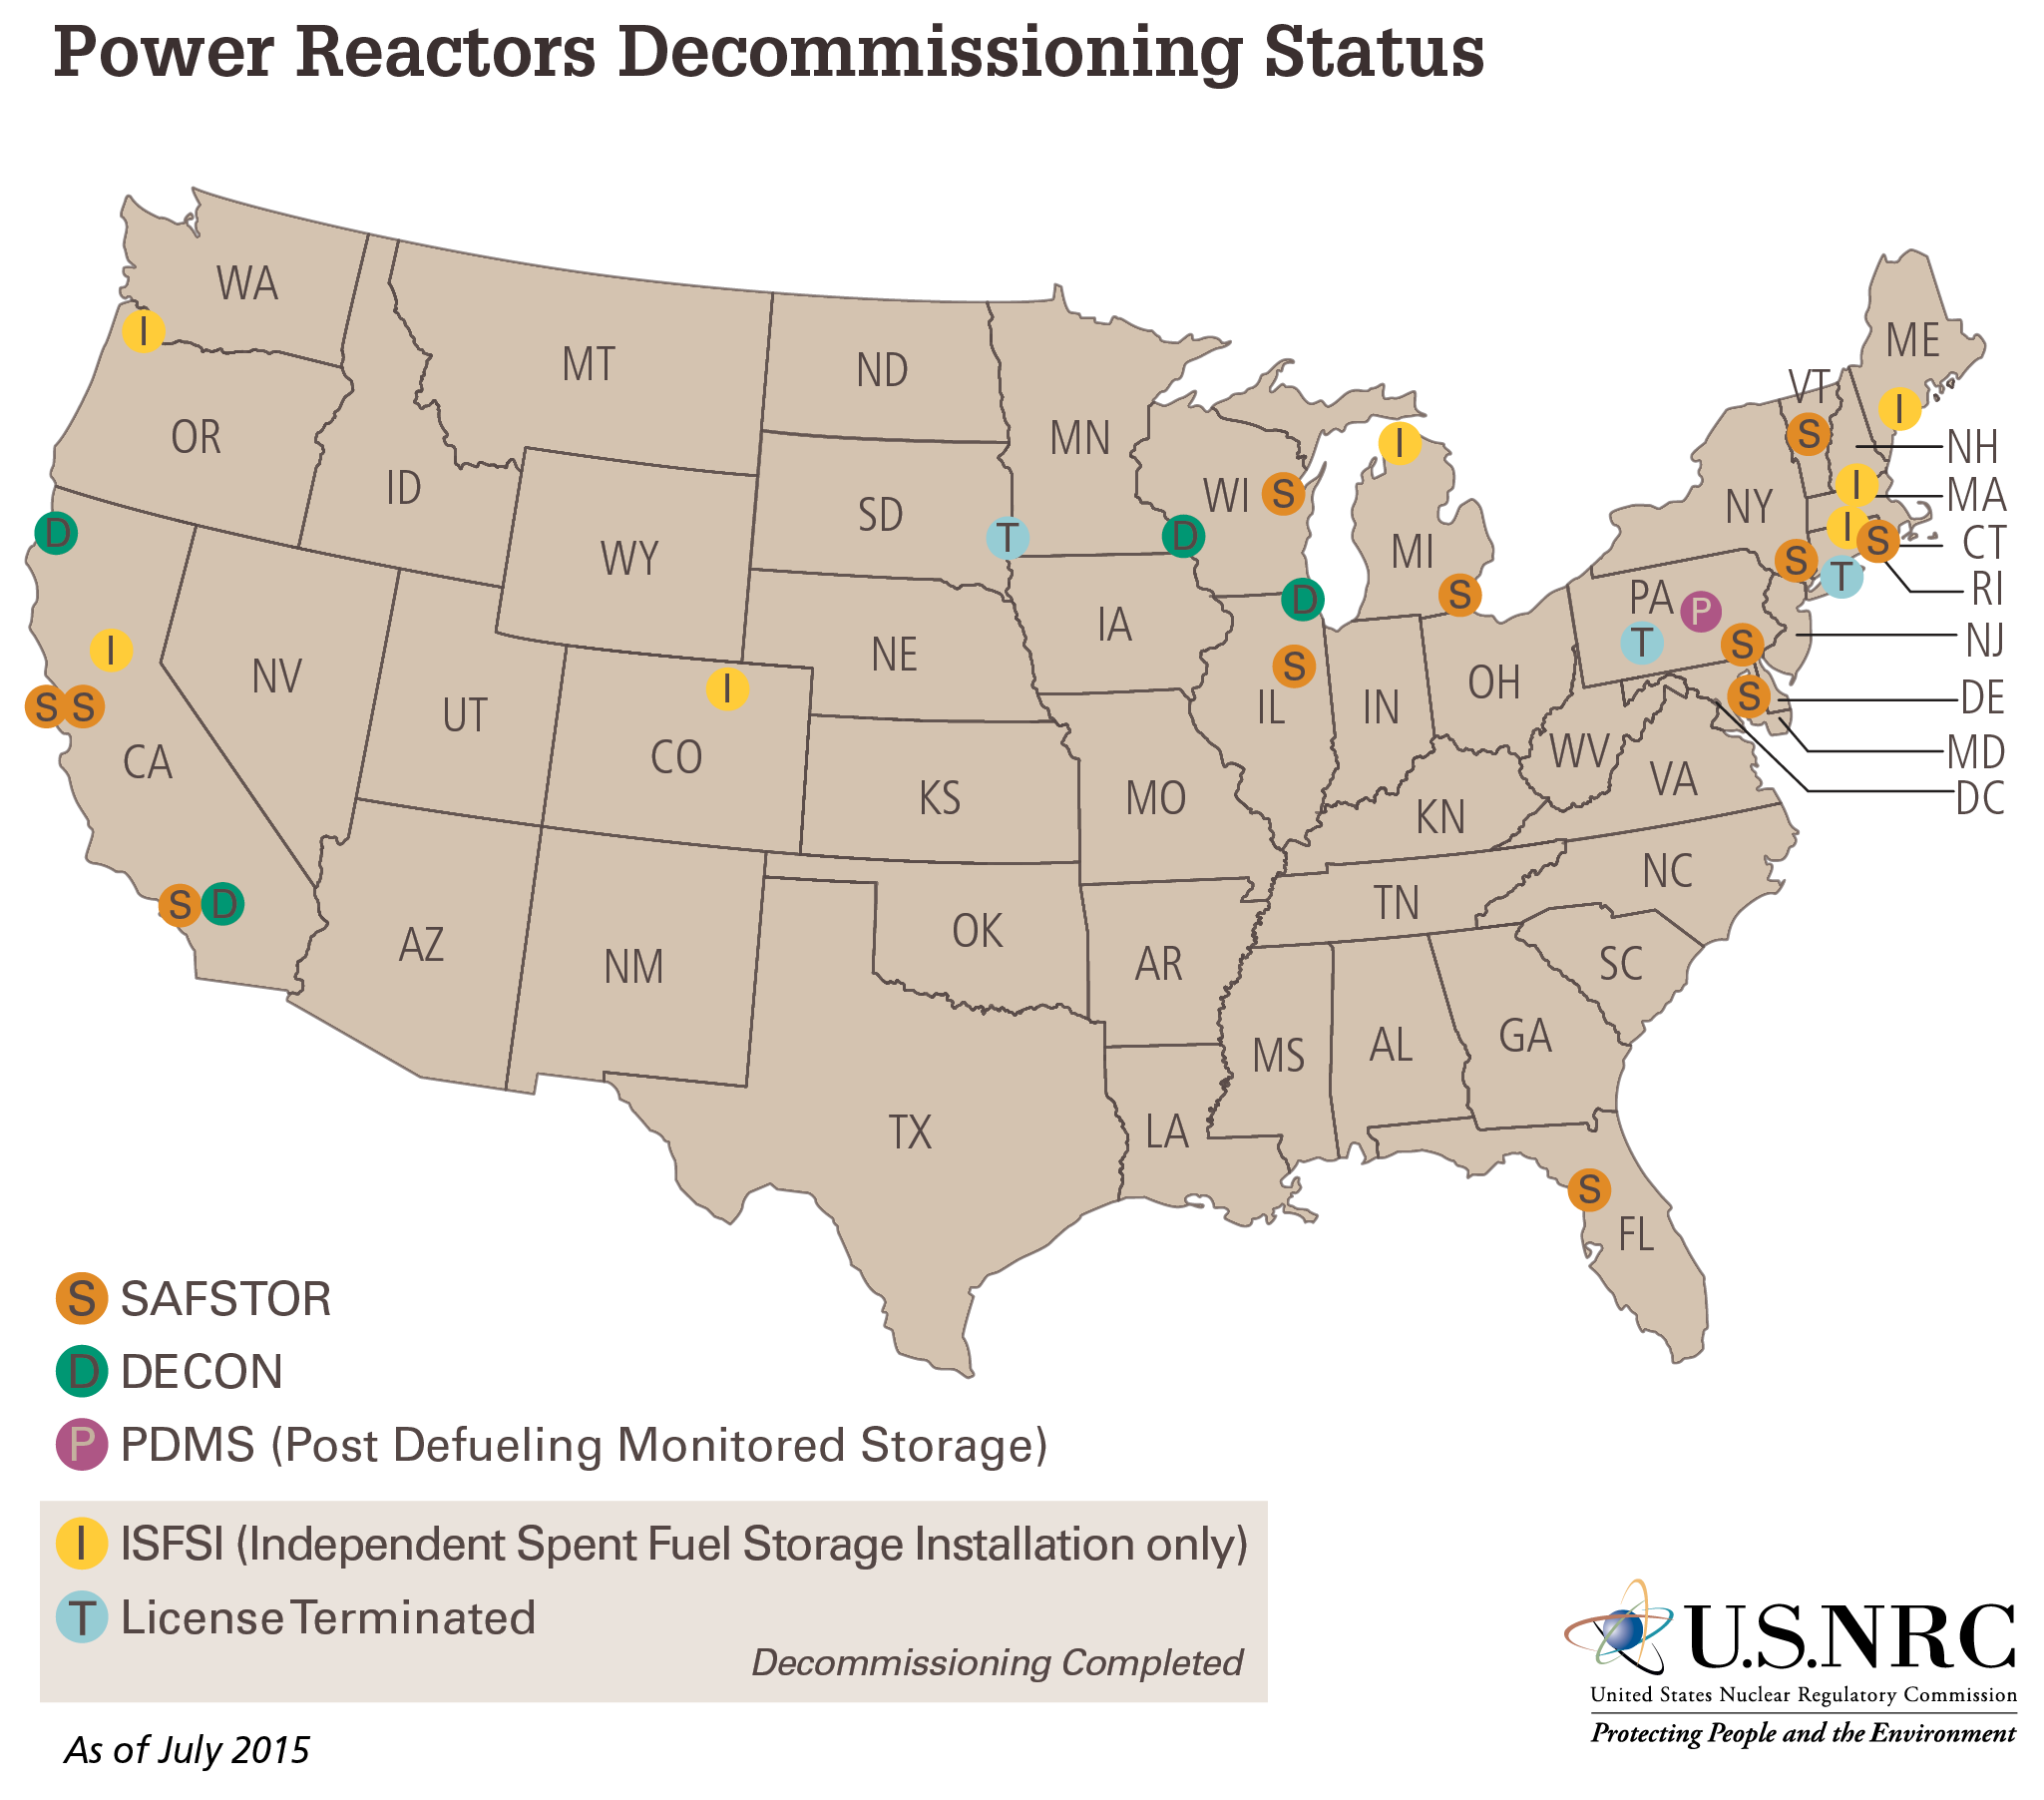
\includegraphics[width=0.8\columnwidth]{power-reactors-decommissioning}	
  \caption{Non-operating facilities status
  \cite{nuclear_regulatory_commission_nrc_2015}.}
  \label{fig:shutdown}
\end{figure}

Finally, integrated siting may be more practically and politically feasible. 
Preliminary work \cite{waleed_regional_2015} indicates integrated siting is 
appealing to many stakeholder groups. For example, a consent-based approval 
process may be feasible because communities local to power plants may be 
uniquely receptive to the incentives of hosting a repository. 

This paper seeks to quantify the impact of these and other features of the 
proposed siting strategy. 

%%%%%%%%%%%%%%%%%%%%%%%%%%%%%%%%%%%%%%%%%%%%%%%%%%%%%%%%%%%%%%%%%%%%%%%%%%%%%%%

\section{Methodology}

This work will evaluate \textbf{3 scenarios} for repository siting according to \textbf{6 metrics} of 
performance considered from the perspective of \textbf{5 stakeholders.}

Preliminary work \cite{waleed_regional_2015} suggests that integrated siting 
will reduce costs, construction, time (both for construction and licensing), 
transportation distances, and resistence from the local community.  
The goal of this paper is to compare this siting strategy with the 
business-as-usual base case via quantitative metrics capturing the key 
priorities of stakeholders. Accordingly, the present 
work will compare three siting scenarios along these axes. 

\begin{itemize}
        \item The reference case: a standalone borehole repository at Yucca Mountain.  
        \item The proposed case: a repository sited at a shutdown reactor site 
                in the midwest.
        \item The combined case: both repositories in operation, burdened only 
                by the \gls{SNF} generated in their half of the US. 
\end{itemize}

 This work will evaluate the potential impacts of each siting strategy according 
to the following 6 quantitative measures:

\begin{itemize}
        \item Transportation Burden $[MTHM \cdot km]$: A site is preferred by 
                most stakeholders if it can minimize the distance \gls{SNF} 
                must travel.
        \item Job Creation $[\#]$: A repository concept is preferred by 
                government and community stakeholders if it is a source of 
                jobs. 
        \item Workforce Utilization $[\$]$: A repository site is preferred by 
                many stakeholders if it utilizes an already skilled local 
                workforce. 
        \item Expediency $[y]$: Many stakeholders will benefit if the removal 
                of dry casks from current storage pads is expedited.
        \item Consent Basis $[\frac{MW}{\mbox{person}}]$: If there is a basis for a consent-based 
                siting process to succeed, many stakeholders benefit.
        \item Site Access $[-]$: Rail access to the site is essential for 
                beginning operations.
        \item Site Appropriateness $[-]$: A site must be geologically 
                appropriate, of sufficient area, etc.
\end{itemize}

Finally, recognizing that these measures are valued differently by each, we
consider possible weighting factors that may capture the perspectives of 5 key
stakeholder groups:

\begin{itemize}
        \item the federal government,
        \item the state government,
        \item the local government,
        \item the local community,
        \item and the owner of the non-operating plant.
\end{itemize}



	\documentclass{anstrans}

%%%% packages and definitions (optional)
\usepackage{graphicx} % allows inclusion of graphics
\usepackage{booktabs} % nice rules (thick lines) for tables
\usepackage{microtype} % improves typography for PDF

\newcommand{\SN}{S$_N$}
\renewcommand{\vec}[1]{\bm{#1}} %vector is bold italic
\newcommand{\vd}{\bm{\cdot}} % slightly bold vector dot
\newcommand{\grad}{\vec{\nabla}} % gradient
\newcommand{\ud}{\mathop{}\!\mathrm{d}} % upright derivative symbol


\title{Benefits of Siting a Borehole Repository on Non-Operating Nuclear 
Facility}
\author{Jin Whan Bae, William Roy, Kathryn Huff}

\institute{
Dept. of Nuclear, Plasma, and Radiological Engineering, University of Illinois at Urbana-Champaign
\and
Urbana, IL
}
\email{jbae11@illinois.edu}


%%%% Acronym support

\usepackage[acronym,toc]{glossaries}
%\newacronym{<++>}{<++>}{<++>}
\newacronym[longplural={metric tons of heavy metal}]{MTHM}{MTHM}{metric ton of heavy metal}
\newacronym{ABM}{ABM}{agent-based modeling}
\newacronym{ACDIS}{ACDIS}{Program in Arms Control \& Domestic and International Security}
\newacronym{AHTR}{AHTR}{Advanced High Temperature Reactor}
\newacronym{ANDRA}{ANDRA}{Agence Nationale pour la gestion des D\'echets RAdioactifs, the French National Agency for Radioactive Waste Management}
\newacronym{ANL}{ANL}{Argonne National Laboratory}
\newacronym{API}{API}{application programming interface}
\newacronym{ASME}{ASME}{American Society of Mechanical Engineers}
\newacronym{ATWS}{ATWS}{Anticipated Transient Without Scram}
\newacronym{BDBE}{BDBE}{Beyond Design Basis Event}
\newacronym{BIDS}{BIDS}{Berkeley Institute for Data Science}
\newacronym{CAFCA}{CAFCA}{ Code for Advanced Fuel Cycles Assessment }
\newacronym{CDTN}{CDTN}{Centro de Desenvolvimento da Tecnologia Nuclear}
\newacronym{CEA}{CEA}{Commissariat \`a l'\'Energie Atomique et aux \'Energies Alternatives}
\newacronym{CI}{CI}{continuous integration}
\newacronym{CNEN}{CNEN}{Comiss\~{a}o Nacional de Energia Nuclear}
\newacronym{CNERG}{CNERG}{Computational Nuclear Engineering Research Group}
\newacronym{COSI}{COSI}{Commelini-Sicard}
\newacronym{COTS}{COTS}{commercial, off-the-shelf}
\newacronym{CSNF}{CSNF}{commercial spent nuclear fuel}
\newacronym{CTAH}{CTAHs}{Coiled Tube Air Heaters}
\newacronym{CUBIT}{CUBIT}{CUBIT Geometry and Mesh Generation Toolkit}
\newacronym{CURIE}{CURIE}{Centralized Used Fuel Resource for Information Exchange}
\newacronym{DAG}{DAG}{directed acyclic graph}
\newacronym{DANESS}{DANESS}{Dynamic Analysis of Nuclear Energy System Strategies}
\newacronym{DBE}{DBE}{Design Basis Event}
\newacronym{DESAE}{DESAE}{Dynamic Analysis of Nuclear Energy Systems Strategies}
\newacronym{DHS}{DHS}{Department of Homeland Security}
\newacronym{DOE}{DOE}{Department of Energy}
\newacronym{DRACS}{DRACS}{Direct Reactor Auxiliary Cooling System}
\newacronym{DRE}{DRE}{dynamic resource exchange}
\newacronym{DSNF}{DSNF}{DOE spent nuclear fuel}
\newacronym{DYMOND}{DYMOND}{Dynamic Model of Nuclear Development }
\newacronym{EBS}{EBS}{Engineered Barrier System}
\newacronym{EDZ}{EDZ}{Excavation Disturbed Zone}
\newacronym{EIA}{EIA}{U.S. Energy Information Administration}
\newacronym{EPA}{EPA}{Environmental Protection Agency}
\newacronym{EP}{EP}{Engineering Physics}
\newacronym{FCO}{FCO}{Fuel Cycle Options}
\newacronym{FCT}{FCT}{Fuel Cycle Technology}
\newacronym{FEHM}{FEHM}{Finite Element Heat and Mass Transfer}
\newacronym{FEPs}{FEPs}{Features, Events, and Processes}
\newacronym{FHR}{FHR}{Fluoride-Salt-Cooled High-Temperature Reactor}
\newacronym{FLiBe}{FLiBe}{Fluoride-Lithium-Beryllium}
\newacronym{GDSE}{GDSE}{Generic Disposal System Environment}
\newacronym{GDSM}{GDSM}{Generic Disposal System Model}
\newacronym{GENIUSv1}{GENIUSv1}{Global Evaluation of Nuclear Infrastructure Utilization Scenarios, Version 1}
\newacronym{GENIUSv2}{GENIUSv2}{Global Evaluation of Nuclear Infrastructure Utilization Scenarios, Version 2}
\newacronym{GENIUS}{GENIUS}{Global Evaluation of Nuclear Infrastructure Utilization Scenarios}
\newacronym{GPAM}{GPAM}{Generic Performance Assessment Model}
\newacronym{GRSAC}{GRSAC}{Graphite Reactor Severe Accident Code}
\newacronym{GUI}{GUI}{graphical user interface}
\newacronym{HLW}{HLW}{high level waste}
\newacronym{HPC}{HPC}{high-performance computing}
\newacronym{HTC}{HTC}{high-throughput computing}
\newacronym{HTGR}{HTGR}{High Temperature Gas-Cooled Reactor}
\newacronym{IAEA}{IAEA}{International Atomic Energy Agency}
\newacronym{INL}{INL}{Idaho National Laboratory}
\newacronym{IPRR1}{IRP-R1}{Instituto de Pesquisas Radioativas Reator 1}
\newacronym{IRP}{IRP}{Integrated Research Project}
\newacronym{ISFSI}{ISFSI}{Independent Spent Fuel Storage Installation}
\newacronym{ISRG}{ISRG}{Independent Student Research Group}
\newacronym{JFNK}{JFNK}{Jacobian-Free Newton Krylov}
\newacronym{LANL}{LANL}{Los Alamos National Laboratory}
\newacronym{LBNL}{LBNL}{Lawrence Berkeley National Laboratory}
\newacronym{LCOE}{LCOE}{levelized cost of electricity}
\newacronym{LDRD}{LDRD}{laboratory directed research and development}
\newacronym{LFR}{LFR}{Lead-Cooled Fast Reactor}
\newacronym{LLNL}{LLNL}{Lawrence Livermore National Laboratory}
\newacronym{LOFC}{LOFC}{Loss of Forced Cooling}
\newacronym{LOHS}{LOHS}{Loss of Heat Sink}
\newacronym{LOLA}{LOLA}{Loss of Large Area}
\newacronym{LP}{LP}{linear program}
\newacronym{MA}{MA}{minor actinide}
\newacronym{MCNP}{MCNP}{Monte Carlo N-Particle code}
\newacronym{MILP}{MILP}{mixed-integer linear program}
\newacronym{MIT}{MIT}{the Massachusetts Institute of Technology}
\newacronym{MOAB}{MOAB}{Mesh-Oriented datABase}
\newacronym{MOOSE}{MOOSE}{Multiphysics Object-Oriented Simulation Environment}
\newacronym{MOX}{MOX}{mixed oxide}
\newacronym{MSR}{MSR}{Molten Salt Reactor}
\newacronym{NAGRA}{NAGRA}{National Cooperative for the Disposal of Radioactive Waste}
\newacronym{NEAMS}{NEAMS}{Nuclear Engineering Advanced Modeling and Simulation}
\newacronym{NEUP}{NEUP}{Nuclear Energy University Programs}
\newacronym{NFCSim}{NFCSim}{Nuclear Fuel Cycle Simulator}
\newacronym{NGNP}{NGNP}{Next Generation Nuclear Plant}
\newacronym{NNSA}{NNSA}{National Nuclear Security Administration}
\newacronym{NPRE}{NPRE}{Department of Nuclear, Plasma, and Radiological Engineering}
\newacronym{NQA1}{NQA-1}{Nuclear Quality Assurance - 1}
\newacronym{NRC}{NRC}{Nuclear Regulatory Commission}
\newacronym{NSF}{NSF}{National Science Foundation}
\newacronym{NSSC}{NSSC}{Nuclear Science and Security Consortium}
\newacronym{NUWASTE}{NUWASTE}{Nuclear Waste Assessment System for Technical Evaluation}
\newacronym{NWTRB}{NWTRB}{Nuclear Waste Technical Review Board}
\newacronym{OCRWM}{OCRWM}{Office of Civilian Radioactive Waste Management}
\newacronym{ORION}{ORION}{ORION}
\newacronym{PARCS}{PARCS}{Purdue Advanced Reactor Core Simulator}
\newacronym{PBAHTR}{PB-AHTR}{Pebble Bed Advanced High Temperature Reactor}
\newacronym{PBFHR}{PB-FHR}{Pebble-Bed Fluoride-Salt-Cooled High-Temperature Reactor}
\newacronym{PEI}{PEI}{Peak Environmental Impact}
\newacronym{PH}{PRONGHORN}{PRONGHORN}
\newacronym{PRKE}{PRKE}{Point Reactor Kinetics Equations}
\newacronym{PSPG}{PSPG}{Pressure-Stabilizing/Petrov-Galerkin}
\newacronym{PyNE}{PyNE}{Python toolkit for Nuclear Engineering}
\newacronym{PyRK}{PyRK}{Python for Reactor Kinetics}
\newacronym{QA}{QA}{quality assurance}
\newacronym{RDD}{RD\&D}{Research Development and Demonstration}
\newacronym{RD}{R\&D}{Research and Development}
\newacronym{RELAP}{RELAP}{Reactor Excursion and Leak Analysis Program}
\newacronym{RIA}{RIA}{Reactivity Insertion Accident}
\newacronym{RIF}{RIF}{Region-Institution-Facility}
\newacronym{SFR}{SFR}{Sodium-Cooled Fast Reactor}
\newacronym{SINDAG}{SINDA{\textbackslash}G}{Systems Improved Numerical Differencing Analyzer $\backslash$ Gaski}
\newacronym{SKB}{SKB}{Svensk K\"{a}rnbr\"{a}nslehantering AB}
\newacronym{SNF}{SNF}{spent nuclear fuel}
\newacronym{SNL}{SNL}{Sandia National Laboratory}
\newacronym{STC}{STC}{specific temperature change}
\newacronym{SUPG}{SUPG}{Streamline-Upwind/Petrov-Galerkin}
\newacronym{SWF}{SWF}{Separations and Waste Forms}
\newacronym{SWU}{SWU}{Separative Work Unit}
\newacronym{TRIGA}{TRIGA}{Training Research Isotope General Atomic}
\newacronym{TRISO}{TRISO}{Tristructural Isotropic}
\newacronym{TSM}{TSM}{Total System Model}
\newacronym{TSPA}{TSPA}{Total System Performance Assessment for the Yucca Mountain License Application}
\newacronym{ThOX}{ThOX}{thorium oxide}
\newacronym{UFD}{UFD}{Used Fuel Disposition}
\newacronym{UML}{UML}{Unified Modeling Language}
\newacronym{UOX}{UOX}{uranium oxide}
\newacronym{UQ}{UQ}{uncertainty quantification}
\newacronym{US}{US}{United States}
\newacronym{UW}{UW}{University of Wisconsin}
\newacronym{VISION}{VISION}{the Verifiable Fuel Cycle Simulation Model}
\newacronym{VV}{V\&V}{verification and validation}
\newacronym{WIPP}{WIPP}{Waste Isolation Pilot Plant}
\newacronym{YMR}{YMR}{Yucca Mountain Repository Site}


	
\makeglossaries




\begin{document}

%%%%%%%%%%%%%%%%%%%%%%%%%%%%%%%%%%%%%%%%%%%%%%%%%%%%%%%%%%%%
\section{Case Definition and Methodology}

A proposed case is building a 70,000 \gls{MTHM} capacity borehole repository at the Clinton Power Plant in Illinois. The base case is to build a standalone borehole repository at a location similar to that of Yucca Mountain with the same capacity. 

\subsection{Proposed Case Methodology and Definition}
The proposed case is siting a borehole repository at a shut-down power plant.
 In order to minimize transport cost, a central location is preferred. An
  elementary analysis on the transportation of spent fuel is done by
   calculating the total amount of waste times the distance it has to travel
    ( in units of MTHM*km). The distance between each storage site 
    (i.e. reactors and \gls{ISFSI}) is calculated by 
    using the havershine formula on the geographical coordinates of the sites. The
     coordinates and spent fuel inventory data
    is from the GC-859 data from the \gls{EIA} %\cite{?????}
    and the \gls{CURIE} website.
     From the list of 74 reactors, several candidates
    with the smallest MTHM*Km value is listed below:
    
    
\begin{table}[h]
\centering
    \caption { Reactors with least MTHM*Km value}
	\begin{tabular}{l|l|l|l}
	\hline
	Reactor & State & $MTHM*km$ & License Area [$km^2$]  \\ \hline
	Clinton & Illinois &  77,352,339 & 57.87   \\ \hline
	Peach Bottom & Pennsylvania & 85,563,135 & 2.509   \\ \hline
	Indian Point &   New York & 77,352,339 & ?????   \\ \hline
	Dresden & Illinois &  77,663,969 & 3.856   \\ \hline
	
	\end{tabular}
\end {table}


The Clinton Power Plant is chosen as the site for the proposed case due to its
low $MTHM*km^2$ value and substantially large license area. Considering that only
 $30km^2$ is required for all the total \gls{SNF} amount, the licensed area at Clinton power plant allows more than  enough space to site a borehole repository, which avoids
  possible conflicts with the community from purchasing and utilizing more land.
  
\subsection{Base Case Methodology and Definition}
The base case is presented in order to demonstrate the cost savings and efficiencies 
that arise from the proposed case. The base case mimics the Yucca Mountain Project
 except the design. Costs include new licensing and processing facility for repacking 
the spent fuel assemblies.

%%%%%%%%%%%%%%% Temporarily disabled Table %%%%%%%%%%%%%%%%%%%%%%%%%%%%%%%
    
\iffalse

\begin{table}[h]
\centering
\caption {Incentive Criterion and Weight for Each Stakeholder}
	\begin{tabular}{l|l|l|l|l|l}
	\hline
	 & Federal & State & Local & Utility & Environmental \\ \hline
	Job Creation &   & 1 & 3 & 1 &   \\ \hline
	Transport[$MTHM*km$] & 2 & 1 & 2 & & 2\\ \hline
	No Need for new treatment license & 2 & & & 1 & \\ \hline
	Emptying Spent Fuel Storage Pools & 3 & & & 3 & \\ \hline
	Net Cost & 3 & & & 3 & \\ \hline
	No New Above-Ground Facility Construction & 3 & & & 3 & \\ \hline
	
	\end{tabular}
\end{table}

\fi



%%%%%%%%%%%%%%% Temporarily disabled Table %%%%%%%%%%%%%%%%%%%%%%%%%%%%%%%

\bibliographystyle{ans}
\bibliography{bibliography}

\end{document}
        \section{Acknowledgments}

This material is based upon work supported by \gls{ACDIS}. Preliminary work was 
conducted in collaboration with the \gls{ISRG} within the \gls{NPRE}. The 
authors are accordingly grateful for guidance by Prof. Clifford Singer.





\bibliographystyle{ans}
\bibliography{bibliography}


\end{document}
